\chapter{Introduction}

\label{Chapter1} % For referencing the chapter elsewhere, use \ref{Chapter1} 

La présentation de projets d'urbanisme ou de planification territoriale auprès du public a toujours été un défi. 

Depuis son apparition, la CAO aide les professionnels du domaine à réaliser des modélisations toujours plus précises et réalistes. 
Malheureusement, le partage de ces modélisations nécessite généralement de créer plusieurs maquettes 3D et de les mettre à disposition. Cela demande d'autant plus de travail et de temps que le projet est complexe, voire inclut différentes étapes (2 ans, 5 ans...) avec en conséquence une multitude de maquettes à réaliser.

\begin{figure}[h]
    \centering
    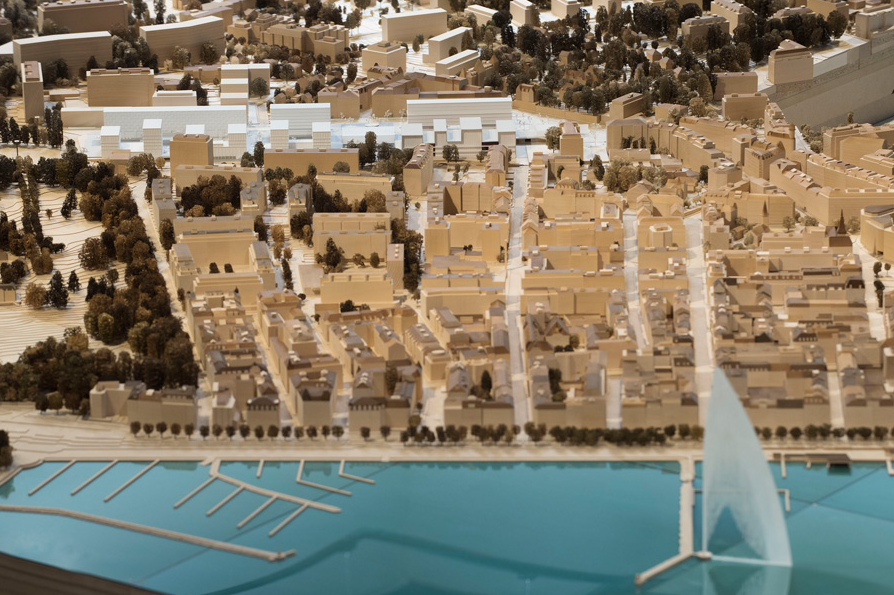
\includegraphics[width=0.8\linewidth]{Figures/geneva-model.png}
    \caption{Maquette de la ville de Genève réalisée à la main.}
    \label{fig:geneva-model}
\end{figure}

L'avènement des imprimantes 3D a permis de réduire cette charge de travail, tout en produisant des maquettes plus fidèles. 


\begin{figure}[h]
    \centering
    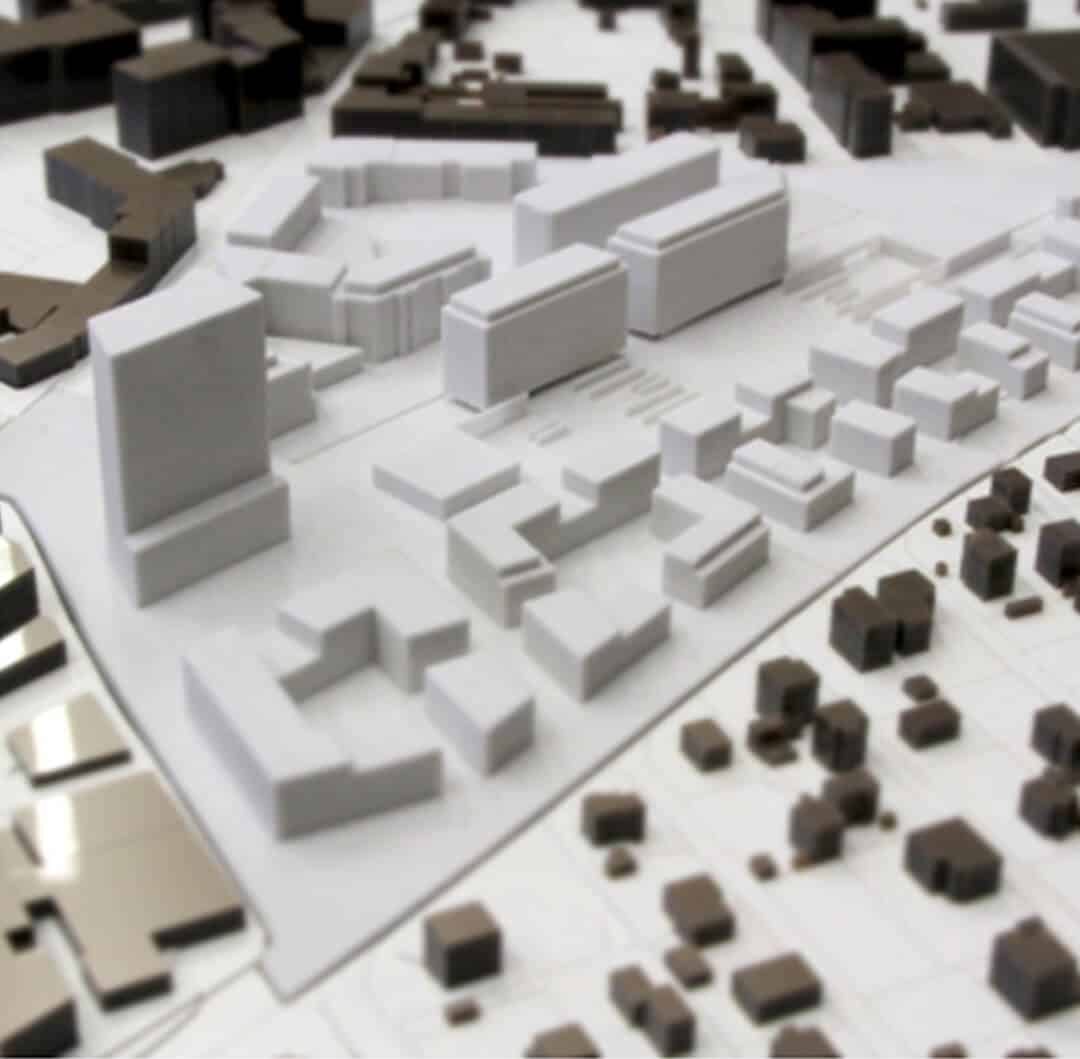
\includegraphics[width=0.5\linewidth]{Figures/3d-printed-model.jpg}
    \captionsource{Exemple de maquette imprimée en 3D.}{3d-printed-model}
    \label{fig:3d-printed-model}
\end{figure}

Un autre problème survient alors: pour voir lesdites maquettes, il faut se rendre à l'endroit où elles sont exposées.

Une solution à cela serait le partage direct des modèles réalisés à l'ordinateur avec les personnes concernées. Cependant, la majorité des projets sont créés à l'aide de logiciels propriétaires, dont la licence est bien souvent très coûteuse (AutoCAD, SketchUp, Cinema4D...). Il n'est dès lors pas envisageable d'exiger des utilisateurs un tel investissement d'argent et de temps (installation, configuration) dans un simple but de consultation des projets.
Bien que certains de ces produits proposent gracieusement une visionneuse, celle-ci est généralement limitée aux formats supportés par l'éditeur.

Fort heureusement, des outils gratuits permettant de visualiser des modèles 3D de toutes sortes, ont fait leur apparition sur le marché ces dernières années. Certains sont proposés gracieusement par les éditeurs des produits cités précédemment, à l'instar d'Autodesk Viewer. D'autres sont des logiciels clients, comme la visionneuse 3D fournie d'office avec Windows 10 ou Open 3D Model Viewer\footnote{\url{www.open3mod.com}}. Enfin, des solutions en ligne sont également disponibles. Celles-ci ont l'avantage de n'exiger aucune installation, et d'être accessibles à la majorité des systèmes d'exploitation, ne nécessitant qu'un navigateur internet.
C'est cette dernière catégorie qui nous intéresse dans le cadre de ce projet.

Parmi les outils en ligne existants, le plus utilisé, et sans doute le plus complet actuellement, se nomme \textbf{Sketchfab}. Plus qu'une simple visionneuse, il s'agit d'une plateforme permettant de stocker, partager et visualiser des modèles 3D. 
%Elle sera détaillée dans la section \ref{sketchfab}.

\section{Sketchfab} \label{sketchfab}

Lancée en 2012, Sketchfab\footnote{\url{www.sketchfab.com}} est une plateforme web d'hébergement de contenus 3D, ne ciblant aucune catégorie particulière : cela va des modèles de petits objets de la vie courante, de personnages, aux modélisations de paysages et lieux complexes.

\begin{figure}
    \centering
    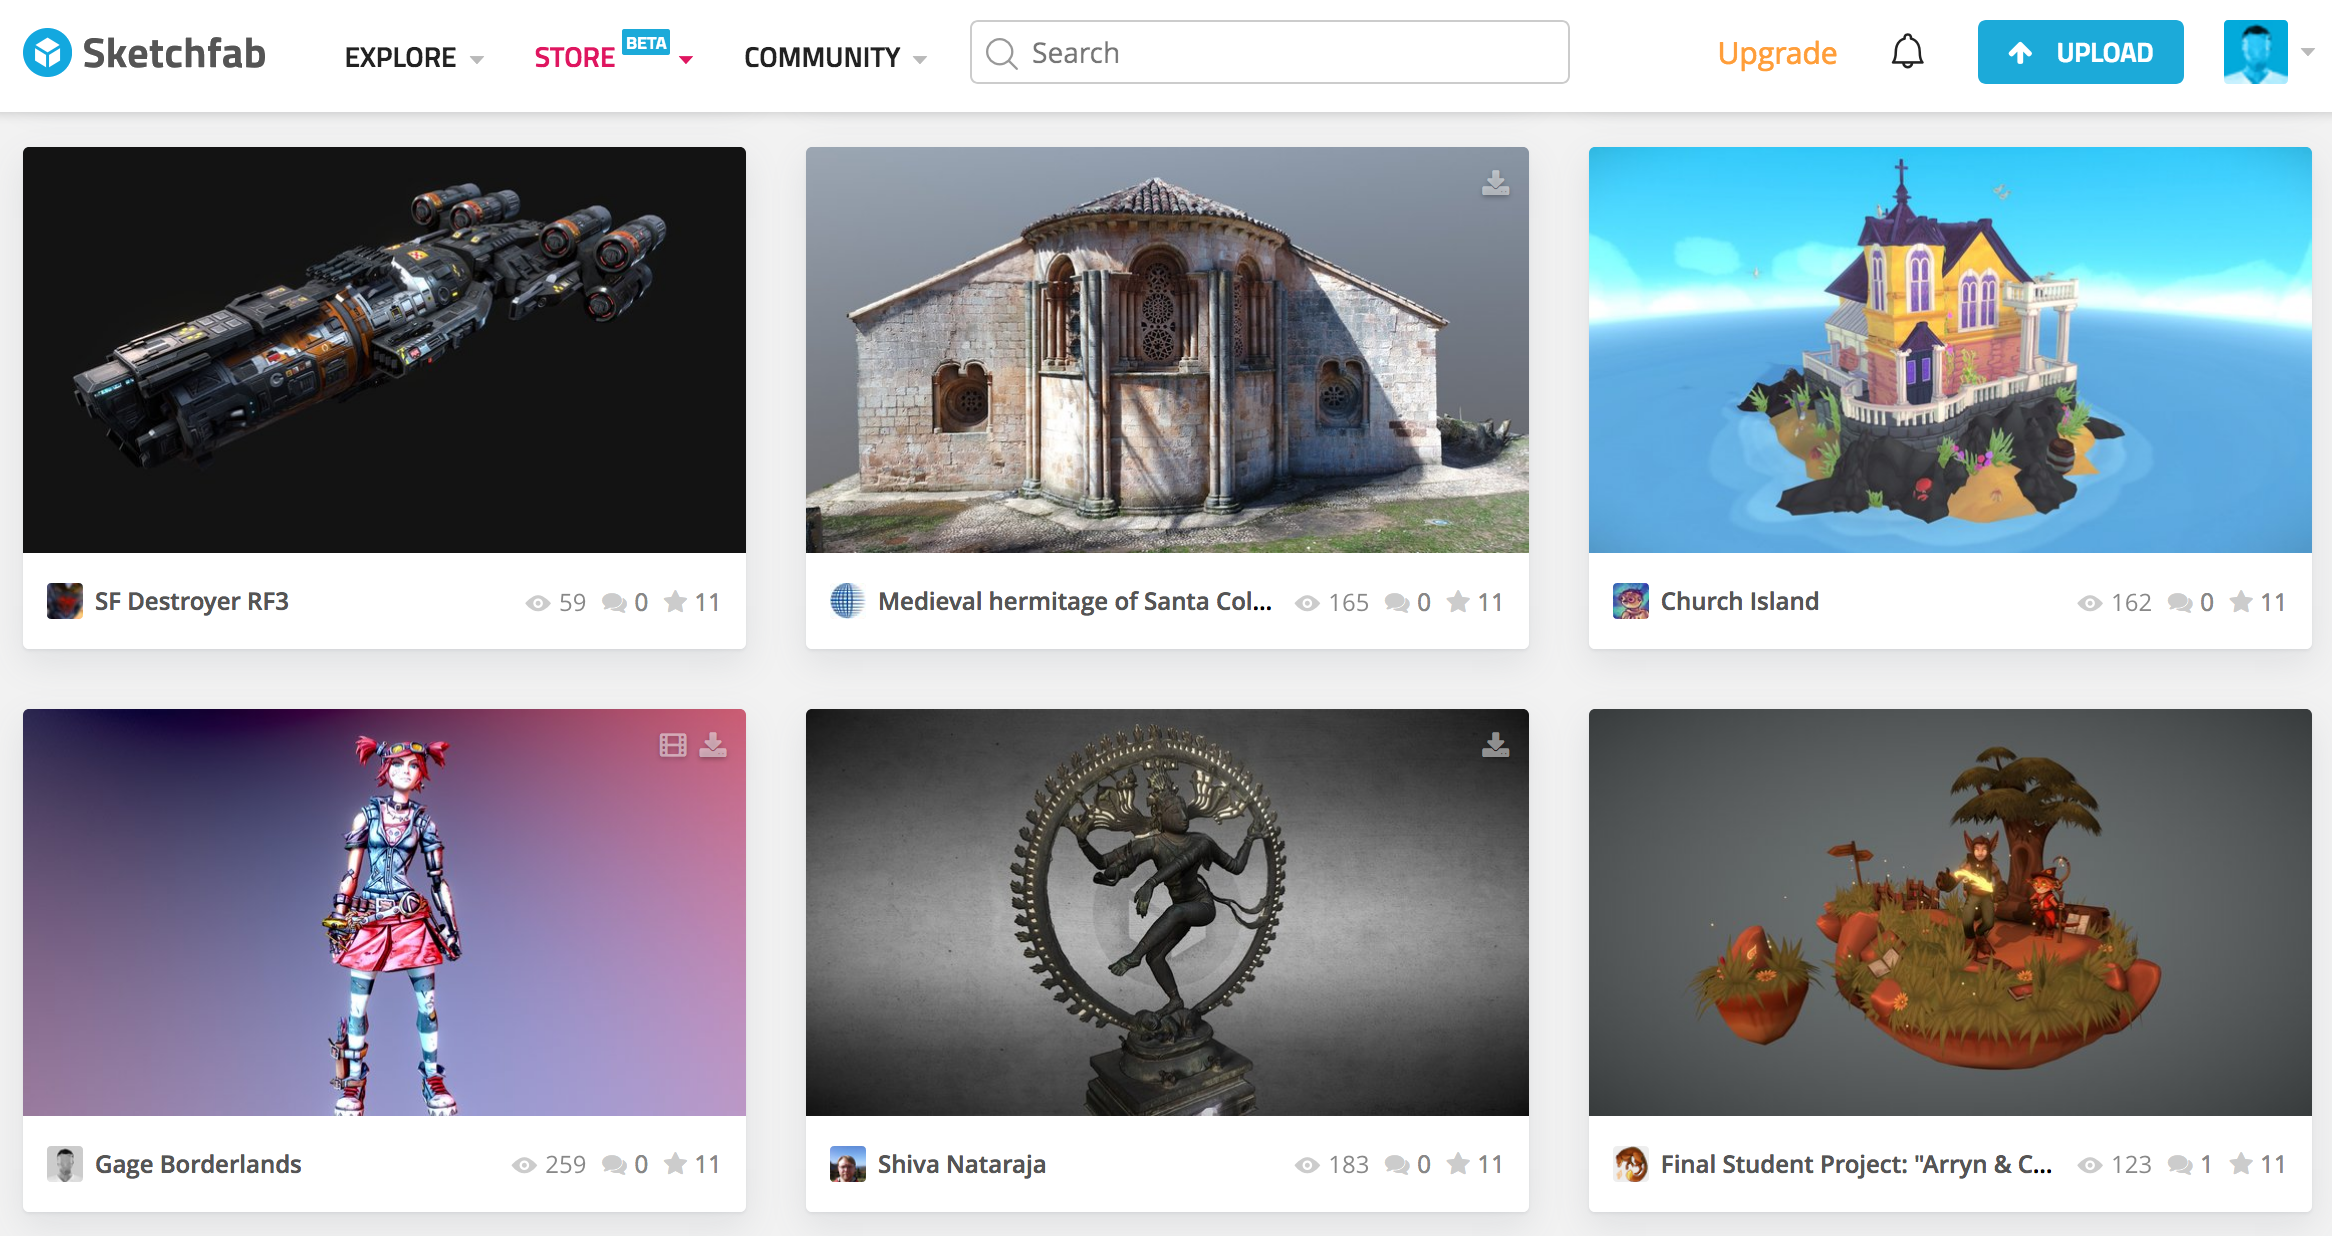
\includegraphics[width=\linewidth]{Figures/sketchfab-overview.png}
    \caption{Affichage de modèles récemments ajouté à Sketchfab.}
    \label{fig:sketchfab-overview}
\end{figure}

Elle permet de visualiser les modèles 3D sur toutes plateformes possédant un navigateur (ordinateurs, smartphones, et même casques de réalité virtuelle).
Il est ainsi possible de naviguer dans le modèle à l'aide d'une souris ou de manière tactile, selon le support. Les opérations "classiques" telles que \textit{zoomer} ou \textit{pivoter} sont disponibles.
Le propriétaire d'un modèle peut également lui adjoindre des annotations. Une annotation est liée à une coordonnée 3D choisie sur le modèle, possède un titre, et peut contenir un texte descriptif ou une image.

\begin{figure}[h]
    \centering
    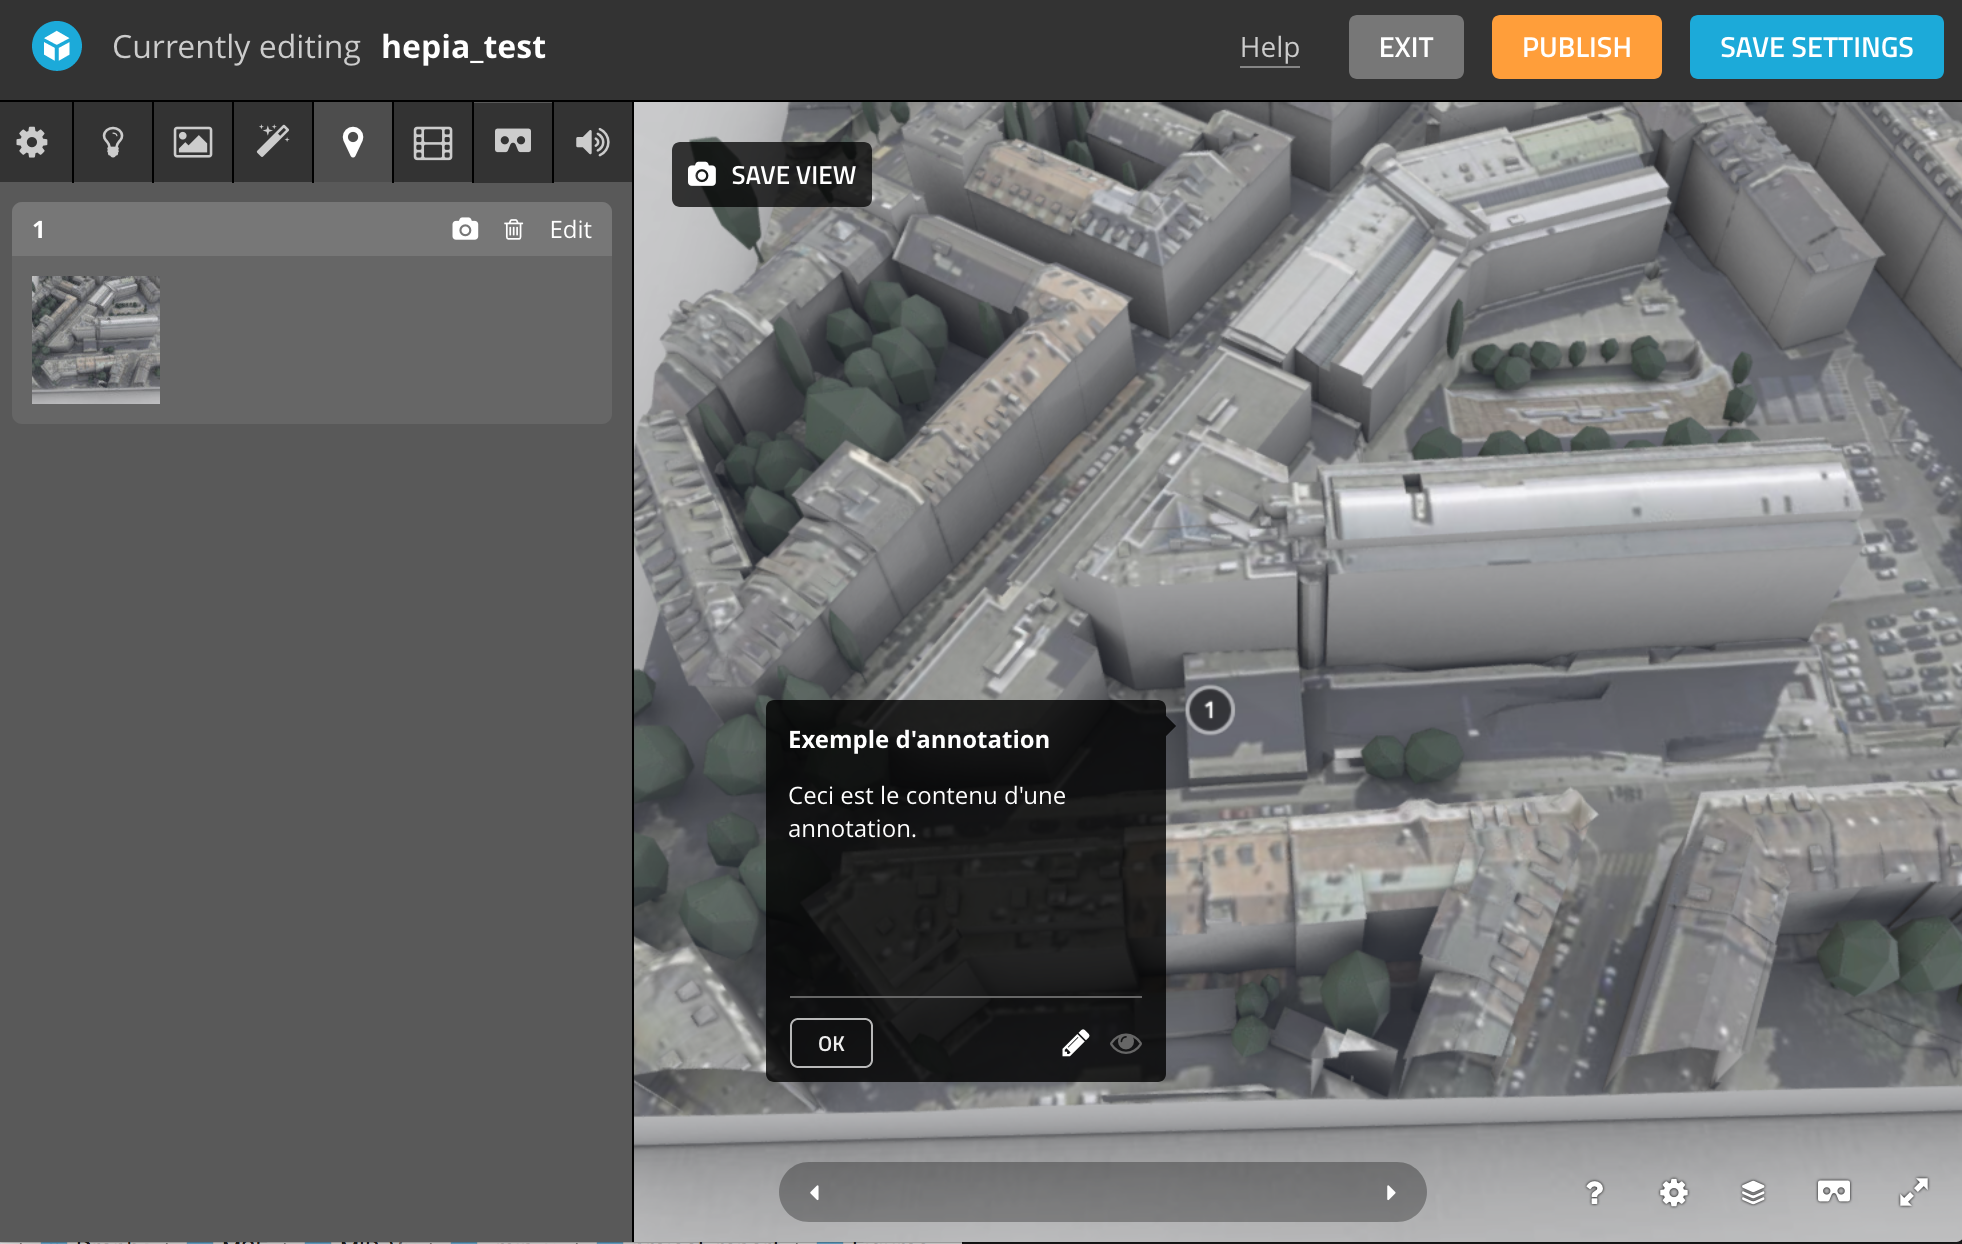
\includegraphics[width=\linewidth]{Figures/sketchfab-annotation-example.png}
    \caption{Ajout d'une annotation à un modèle dans Sketchfab.}
    \label{fig:sketchfab-annotation-example}
\end{figure}

Sketchfab propose plusieurs niveaux de fonctionnalités \footnote{\url{https://sketchfab.com/plans}}. Les principales limitations de l'offre gratuite sont:
\begin{itemize}
    \item Les modèles ajoutés sont obligatoirement référencés et publiques; il n'est pas possible d'en restreindre l'accès.
    \item La taille maximale d'un modèle est de 50 Mo, contre plusieurs centaines de Mo avec une offre payante, ce qui est assez restreignant.
    \item Seules 5 annotations peuvent être ajoutées à un modèle.
\end{itemize}

Récemment, la plateforme a mis en place un \textit{store} (encore en version \textit{beta}) permettant de vendre et acheter des modèles, généralement un peu plus complexes et travaillés.

\section{Problématique}

À la Haute école du paysage, d'ingénierie et d'architecture de Genève (hepia), le groupe de modélisation informatique du paysage\footnote{Groupe MIP, institut inPACT, \url{https://mip.hesge.ch}} (MIP) manifeste un intérêt marqué pour un tel outil dans le cadre de ses mandats. En intégrant une telle plateforme dans ses processus, le partage et l'accès aux modélisations pour les acteurs concernés s'en trouveraient facilité.

\textit{Sketchfab} présente néanmoins des lacunes. Pour commencer, citons les limitations évoquées dans la section~\ref{sketchfab}, malgré l'option plus ou moins satisfaisante de la formule payante.
S'agissant d'une plateforme généraliste, elle n'offre pas certains outils spécifiques, propres au domaine de l'urbanisme. D'autres inconvénients, comme le manque de personnalisation (par exemple, pouvoir isoler les divers modèles relatifs à un projet), les droits d'accès (gérer les personnes autorisées à consulter un groupe de modèles, ainsi que les possibilités d'interactions de chacun).

Concernant les annotations, rappelons que leur nombre est limité à cinq pour la formule gratuite, et qu'elles ne peuvent contenir que du texte et des images (celles-ci devant alors être hébergées ailleurs). En outre, la description ne peut dépasser 1024 caractères.

Idéalement, il faudrait pouvoir bénéficier d'une plateforme similaire à \textit{Sketchfab}, mais répondant aux besoins spécifiques du domaine de l'aménagement du territoire, tout en offrant la possibilité d'être aisément personnalisable.

\section{Objectifs}

Le but général du présent projet est d'étudier la faisabilité et les problématiques de mise en place d'une telle plateforme à vocation collaborative.

Suite à des discussions avec le Prof. Olivier Donzé pour cibler les besoins du groupe MIP, et en tenant compte du temps limité à disposition, l'accent est mis sur les tâches suivantes:
\begin{itemize}
    \item Définir l'architecture de la plateforme.
    \item Déterminer et présenter des cas d'utilisation.
    \item Rechercher et étudier les solutions existantes qui pourraient servir à composer les différentes "briques" du logiciel.
    \item Etudier les technologies de visualisation de maquettes numériques 3D.
    \item Réaliser, si possible, un prototype ou des illustrations à des fins démonstratives.
\end{itemize}

L'architecture se voudra modulaire, afin de pouvoir bien distinguer chaque composant fonctionnel.

Enfin, les possibilités concernant les annotations, notamment le contenu qu'elles peuvent proposer, seront mises en évidence. 
Il s'agit en effet d'un outil particulièrement pratique, et souvent évoqué lors des dicussions autour du sujet de ce travail.

\section{Réalisation}

Le résultat de ce travail est une étude appronfondie des différentes briques pouvant composer une plateforme de modélisation 3D avec gestion d'annotations, destinée particulièrement au secteur de l'urbanisme.

Pour chaque fonctionnalité, des recherches ont été réalisées afin de découvrir si des solutions libres existaient, notamment sur les principaux dépôts de code comme \textit{GitHub} ou \textit{GitLab}. Le cas échéant, celles-ci ont été analysées (librairies et technologies utilisées) afin de déterminer dans quelle mesure il serait envisageable de les utiliser, en association avec d'autres, pour rapidement implémenter un prototype démontrant la faisabilité de mise en place d'une telle plateforme.

Une version de démonstration a justement été développée afin d'illustrer cette utilisation de modules existants et les possibilités d'améliorations éventuelles. Un bilan et des perspectives d'évolution sont également disponibles et viennent ainsi compléter le démonstrateur.

\begin{figure}[h]
    \centering
    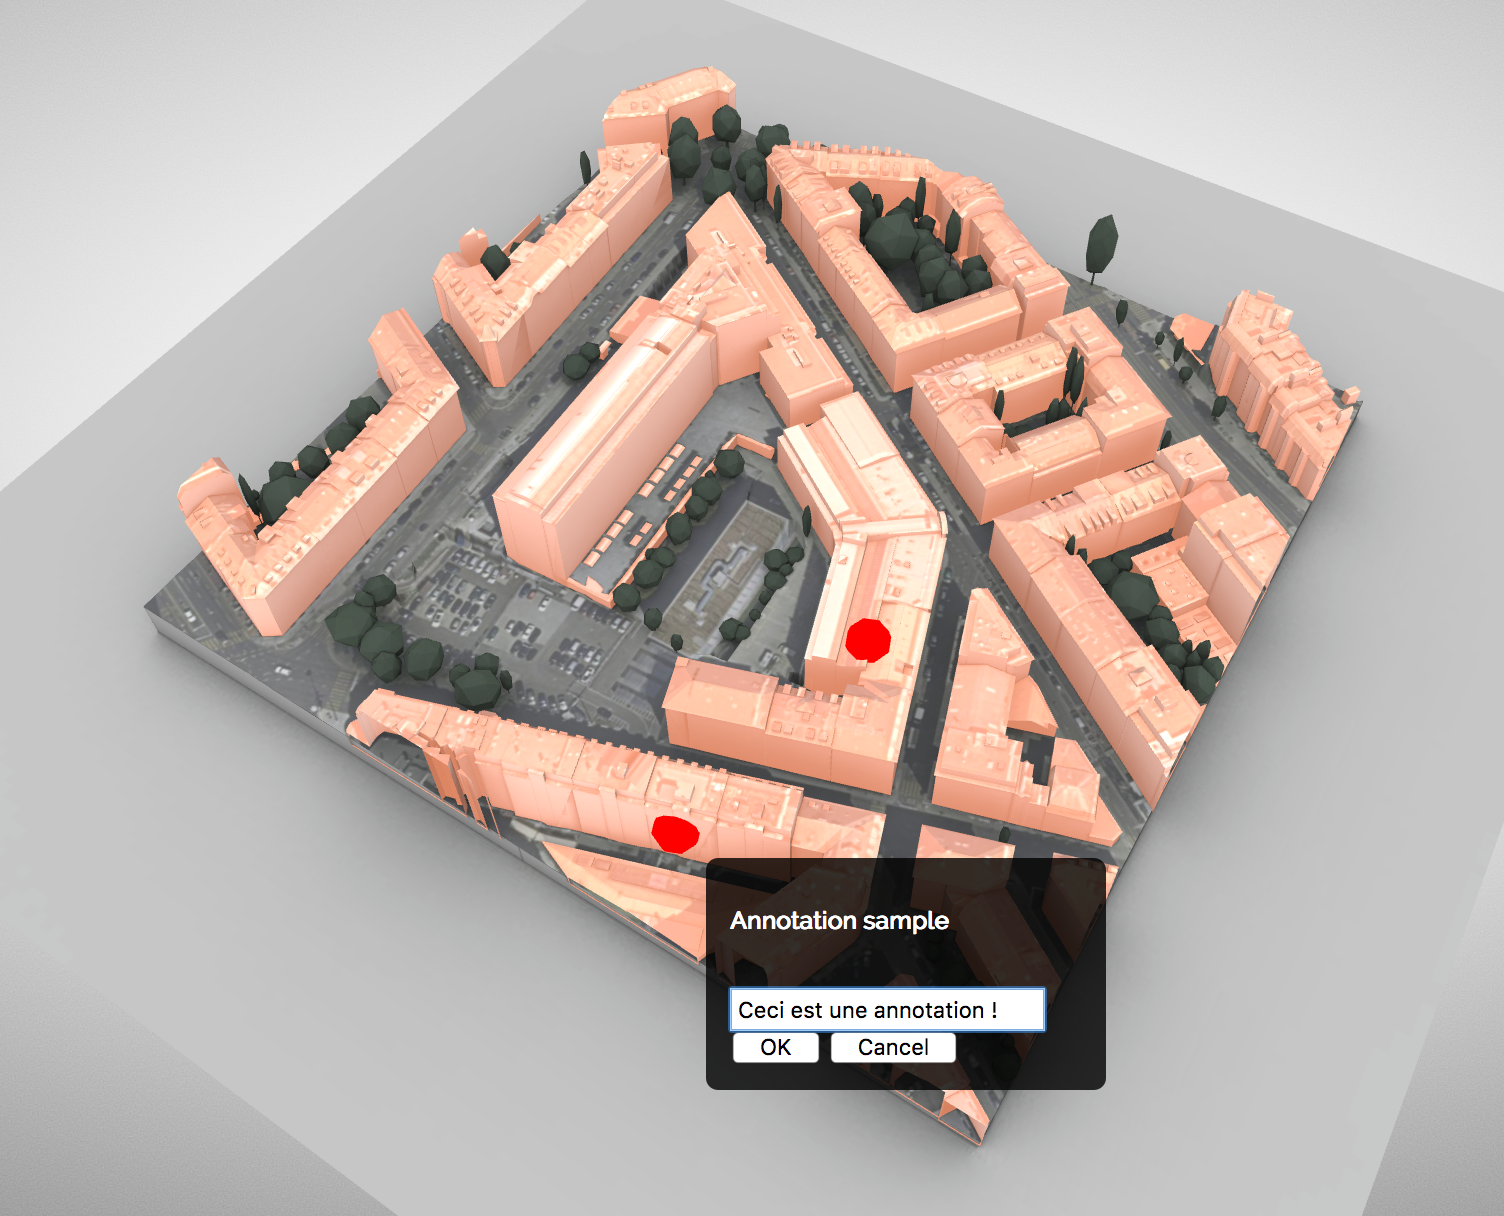
\includegraphics[width=\linewidth]{Figures/mip-viewer-overview.png}
    \caption{"MIP-Viewer", le prototype réalisé: ajout d'annotation sur un modèle importé.}
    \label{fig:mip-viewer-overview}
\end{figure}

L'ensemble du projet (prototype, rapport, illustrations...) est disponible sur GitHub à l'adresse : \textbf{\url{https://github.com/MichaelPolla/mip-viewer/}}

